\documentclass[11pt]{article}

\usepackage{amssymb}
\usepackage{amsmath}
\usepackage{graphicx}
\usepackage{cite}
%\usepackage{algorithmic}
%\usepackage{algorithm}
\usepackage{todonotes}
\usepackage{url}
\usepackage{tikz}
\usetikzlibrary{arrows}

\usepackage{caption}
\usepackage{subcaption}


\usepackage{listings}
 \lstset{
            language=Matlab,                                % choose the language of the code
    %       basicstyle=10pt,                                % the size of the fonts that are used for the code
            numbers=left,                                   % where to put the line-numbers
            numberstyle=\footnotesize,                      % the size of the fonts that are used for the line-numbers
            stepnumber=1,                                           % the step between two line-numbers. If it's 1 each line will be numbered
            numbersep=5pt,                                  % how far the line-numbers are from the code
    %       backgroundcolor=\color{white},          % choose the background color. You must add \usepackage{color}
            showspaces=false,                               % show spaces adding particular underscores
            showstringspaces=false,                         % underline spaces within strings
            showtabs=false,                                         % show tabs within strings adding particular underscores
    %       frame=single,                                           % adds a frame around the code
    %       tabsize=2,                                              % sets default tabsize to 2 spaces
    %       captionpos=b,                                           % sets the caption-position to bottom
            breaklines=true,                                        % sets automatic line breaking
            breakatwhitespace=false,                        % sets if automatic breaks should only happen at whitespace
            escapeinside={\%*}{*)}                          % if you want to add a comment within your code
}

\setlength{\paperwidth}{8.5in}
\setlength{\paperheight}{11in}
\setlength{\voffset}{-0.2in}
\setlength{\topmargin}{0in}
\setlength{\headheight}{0in}
\setlength{\headsep}{0in}
\setlength{\footskip}{30pt}
\setlength{\textheight}{9.25in}
\setlength{\hoffset}{0in}
\setlength{\oddsidemargin}{0in}
\setlength{\textwidth}{6.5in}
\setlength{\parindent}{0in}
\setlength{\parskip}{9pt}

\newcommand{\ben}{\begin{enumerate}}
\newcommand{\een}{\end{enumerate}}

\DeclareGraphicsRule{.JPG}{eps}{*}{`jpeg2ps #1}

\title{Streaming Graph Partitioning Progress Update}
\author{Casey Battaglino\\Robert Pienta}
\date{}
\begin{document}
\maketitle
\section*{Introduction} \vspace{-10 pt}
We have been investigating methods for streaming graph partitioning from simple heuristics to more elaborate approaches like MSR's FENNEL.

We implemented several algorithms in MATLAB and tested them with on synthetic graphs. 
We measured the overall quality of partitions by the \textit{fraction of cut edges} $\lambda$.
\[\lambda = \frac{\text{Number of edges cut by partition}}{\text{Total number of edges}}\]

We investigated the results for the simplest case of partition, the bi-partition or 2-partition, but will continue our tests onto generic k-partitions.  
We have also performed an analysis of the parameters used by FENNEL.

\section*{Synthetic Tests} \vspace{-10 pt}
Our initial tests focus on the partitioner FENNEL which purports to have comparable performance in the quality of partitions with METIS, but with drastically faster computation time on large graphs.

\begin{figure}[ht]
\centering
\caption{A sample adjacency matrix for a partitioned ER graph (n=1000, m=1962), $\gamma = 1.5$}
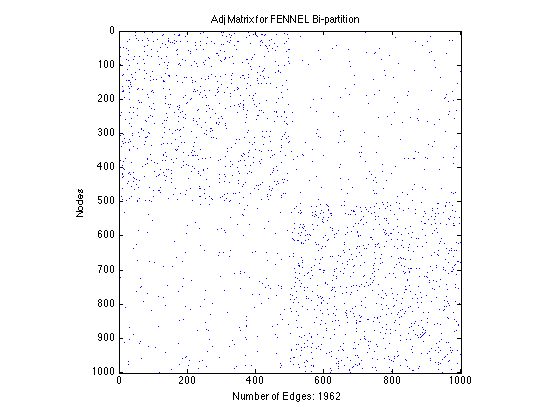
\includegraphics[scale=.65] {figures/adj_spy.png}
\end{figure}

\subsection*{FENNEL} \vspace{-10 pt}
We examined the quality of FENNEL partitions over ER graphs with 1000 nodes and variable numbers of edges.
Each point is the average of multiple ER graph partitions.
\begin{figure}[ht]
\caption{FENNEL experiments investigating partition quality versus graph density and parameter choice.} 
\begin{subfigure}[b]{0.5\textwidth}
\caption{Average $\lambda$ of partition compared against varied density ER graphs (n=1000).  FENNEL's performance quickly degrades as the random graph grows in edge-density.}
\label{figure:quality}
\centering
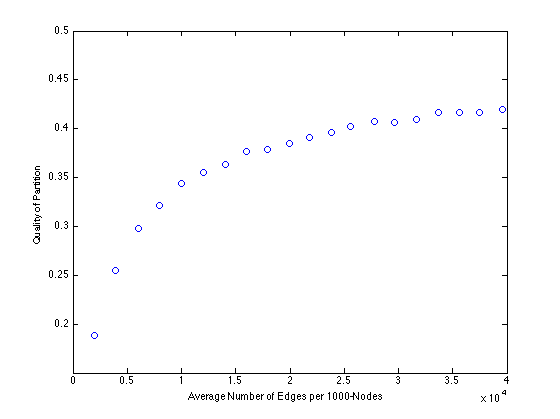
\includegraphics[width=\textwidth] {figures/varied_er_p.png}
\end{subfigure}
\begin{subfigure}[b]{0.5\textwidth}
\caption{Average $\lambda$ of partition compared against varied $\gamma$ for ER graph (n=1000, p=0.001)  The results on $(1,2)$ do not yield differences in performance on ER Graphs.}
\label{figure:gamma}
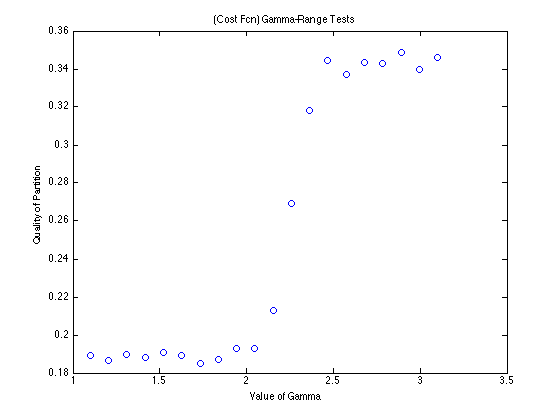
\includegraphics[width=\textwidth] {figures/varied_gamma.png}
\end{subfigure}
\end{figure}
FENNEL uses a deterministic greedy partitioner penalized via a cost function of the form $c(x) = \alpha x^\gamma$.
For $1\le\gamma\le 2$ the cost function balances between adding the new vertex to the partition with the largest number of neighbors and the least number of non-neighbors respectively.
Next we investigated the input parameters to the FENNEL costs function in Figure \ref{figure:quality}.  

Note that in Figure \ref{figure:gamma}, the increase in the cost function past a quadratic incurs a sharp loss in quality as it very heavily suggests the placement of vertices into partitions with the lowest number of non-neighbors.

We tested two suggestions for $\alpha$ with multiple runs on ER graphs.
The results shown in Table \ref{table:qualityalpha}
\begin{table}[ht]
\centering
\caption{The quality of partitions by choice of $\alpha$}
\label{table:qualityalpha}
\begin{tabular}{r | r}\hline
Graph & Ave $\lambda$ \\ \hline &\\
$\sqrt{2}\frac{m}{n^1.5}$ & 18.17\\ &\\
$\vspace{3pt}m\frac{2^\gamma-1}{n^\gamma} $&18.37\\
\end{tabular}
\end{table}



In order to test scale-free distributions we chose to use Kronecker generated scale free network with $n=8192, m=16384$.

\begin{table}[h]
\centering
\caption{The quality of partitions}
\label{table:quality}
\begin{tabular}{r | c}\hline
Graph & $\lambda$ \\ \hline
ER & \\
Kronecker Scale-Free & 30.80\\
others & etc..\\
\end{tabular}
\end{table}

\bibliographystyle{plain}
\bibliography{bib}


\end{document}